%!TEX root=../../../template.tex
\subsection{Tomosim}%
\label{sub:methods_tomosim}

Tomosim is the software program designed for the simulation of the image
reconstruction process in the proposed atmospheric monitoring system of
this dissertation. It corresponds to the last box of the schematic
presented in Figure~\ref{fig:general_system_schematic}. The general
workflow of this piece of software can be viewed in
Figure~\ref{fig:tomosim_start} and
Figure~\ref{fig:tomosim_reconstruction}.

\begin{figure}[htpb]
    \centering
    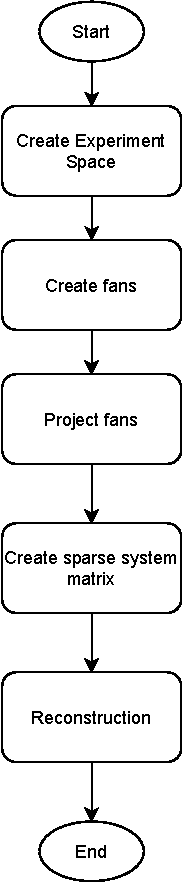
\includegraphics[width=.1\textwidth]{img/pdf/tomosimStartFlowchart.pdf}
    \caption{A flowchart describing the beginning stages of the Tomosim
    simulation.}%
    \label{fig:tomosim_start}
\end{figure}

\begin{figure}[htpb]
    \centering
    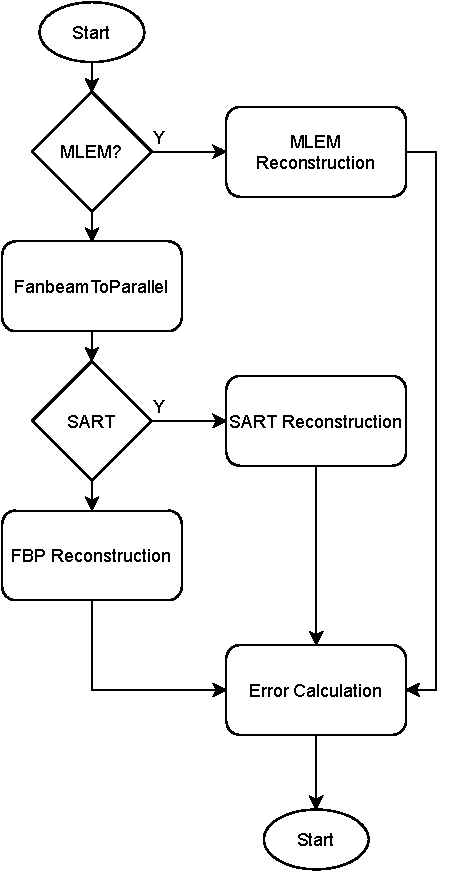
\includegraphics[width=.4\textwidth]{img/pdf/tomosimReconstructionFlowchart.pdf}
    \caption{Flowchart representing the Tomosim operation during the
    reconstruction phase.}%
    \label{fig:tomosim_reconstruction}
\end{figure}


One of the main goals of this piece of software is the evaluation and
characterisation of possible drone trajectories that allow the capture
of sufficient projection data to perform the tomographic inversion. The
trajectory is a key element of the system, as it determines basically
everything in the experiment, and most prominently, its tomographic
geometry. Currently, Tomosim can only use one type of geometry. This is
the fanbeam geometry, as described in
Section~\ref{sec:tomographic_algorithms_and_reconstruction_techniques}.
It was chosen because it seemed to be more promising taking into account
the several important restrictions that this system imposes, namely in
terms of flight time reduction. In essence, the drone's trajectory
(illustrated in
Figure~\ref{fig:illustriated_trajectory_and_fanbeam_formation}) is a
horizontal circle which is parametrised to be at a certain height and to
have a certain diameter.  Both of these dimensions are set at experiment
/ measurement time. The drone stops on this circle at regular angular
intervals, say $\alpha$ degrees. Each one of these stops (360 / $\alpha$
stops) will generate a fanbeam projection, by pointing the optical
system inwards (with respect to the circular macro-trajectory) and
performing a series of spectroscopic measurements in different
directions and also at regular intervals, say $\gamma$ degrees. The
particular case in which $\alpha = \gamma$ is very interesting, because
it then opens the possibility for resorting the fanbeams into parallel
virtual-projections that are much easier to reconstruct tomographically,
as introduced in
Section~\ref{sec:tomographic_algorithms_and_reconstruction_techniques}.  

\begin{figure}[htpb]
    \centering
    \begin{tikzpicture}
        \def\circRad{4}
        \def\d{5}
        \def\noOfRays{3}
        \def\nfans{5}

        \pgfmathsetmacro\width{\circRad*2 + 4}
        \pgfmathsetmacro\nloop{\nfans-1}

        \clip[draw](0,0)circle(\circRad);
        \node[](image) at (0,0)
            {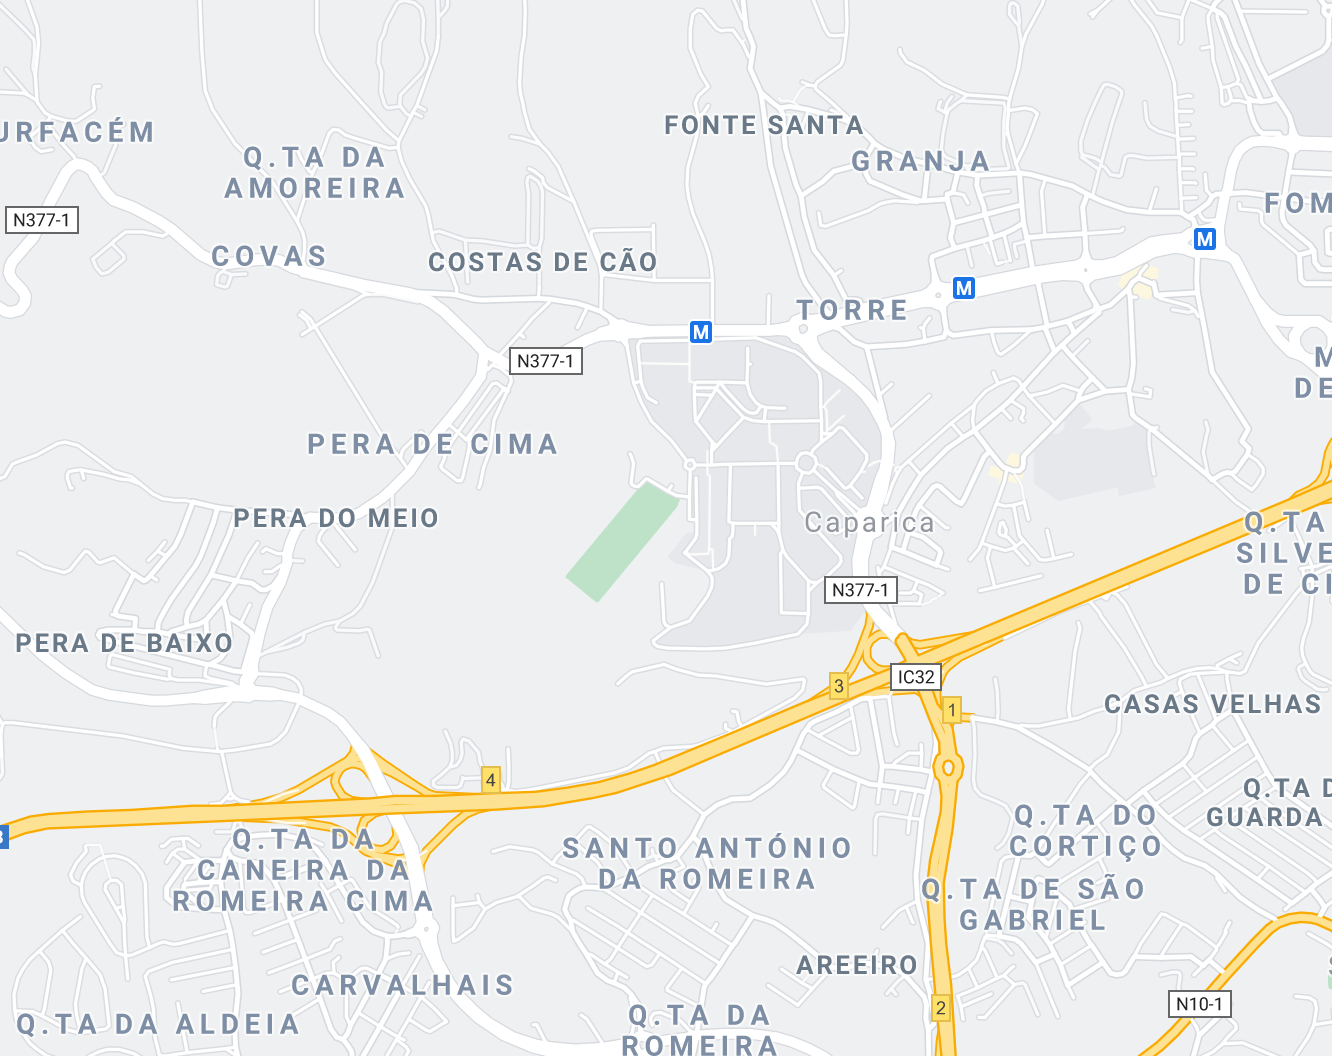
\includegraphics[width=\width cm]{img/png/caparica.png}};
        \draw[name path=c1, color=black, very thick](0,0)circle(\circRad);

        \foreach \fan in {0,...,\nloop}
        {
            \pgfmathsetmacro\pct{(5-\fan)*20}
            \begin{scope}[rotate=\d * \fan, color=black!\pct]
                \node[xshift=.1cm] (A) at (0:\circRad){};
                \foreach \ray in {-\noOfRays,...,\noOfRays}{
                    \path[thin, name path=line] (A)--++(\ray*\d:-13cm);
                    \draw[name intersections={of=line and c1, by={P1}}] (A)--(P1);
                }                
            \end{scope}

        } 
    \end{tikzpicture}

    \caption{ Illustration of the projection gathering algorithm based
    on the assembly of groups of acquisitions as fanbeam projections.
    The lines presented on the drawing come from the right to the left. Each
    is a ray in fan, corresponding to one stop of the drone. In the second
    measurement moment, the drone moves to the exit point on the left and
    repeats the first moment collection. Here, both fans ans rays are
    separated by 5 degrees and there are 6 rays within each fan. A "real
    life" acquisition would feature a lot more rays, but that would be
    graphically complicated for the reader. Both ray and fan angular
    distance are customisable at runtime. Map taken from Google Maps in
    2019. \textsuperscript{\textcopyright}Google.}
    \label{fig:illustriated_trajectory_and_fanbeam_formation}
\end{figure}

Of course, since we want to calculate molecular density in a give
geographic region, we need to delimit our measurements to this space.
The system is able to calculate the point where a given ray of light
exits our \gls{ROI} from the point of entry and its
direction.Figure~\ref{fig:p2_calculation} is a schematic snapshot of a
point in which the drone is taking a spectrum in one of its stops. Here,
the drone's position ($P_1$) is given by the distance $D$ and the angle
$\beta$. The gimbal is pointing at a direction at an angular distance of
$\gamma$ form line $0P_1$. Point $P_2$, which is not known, is at the
intersection between the trajectory's circumference and line $P_1P_2$.
Now, any point on this line can be expressed parametrically, with the
sum of a point and a vector; while to say a point is on a circumference
is the same as saying the distance between that point and the centre of
this circumference is equal to its radius. The situation can be
described by the expressions in Equation~\ref{eq:vectorialLineP1P2}.

\begin{equation}
    \label{eq:vectorialLineP1P2}
    \begin{aligned}
        X &= P_1 + t \cdot (P_2 - P_1)\\
    |P_2| &= D^2\\ 
    \end{aligned}
\end{equation}

Unravelling these expressions, and making use of the algebraic property
that says that $|A|^2 = A \cdot A$, the expression becomes a second
degree equation, as stated in Equation~\ref{eq:secondDegreeEquation},
writing $P_2 - P_1$ as V.

\begin{equation}
    \label{eq:secondDegreeEquation}
    t^2V^2 + 2 \cdot V \cdot P_1 \cdot t + P_{1}^2 - D^2 = 0
\end{equation}

If line $P_1P_2$ non-tangentially intersects the circumference, solving
Equation~\ref{eq:secondDegreeEquation} renders two values for $t$ (which
correspond to $P_1$ and $P_2$). Selection is made by determining the
returned value of $t$ which maximises the euclidean distance between the
produced point and $P_1$.


\begin{figure}[htb]
    \centering
    \includegraphics[width = .8\textwidth]{img/pdf/finding_p2.pdf}
    \caption{$P_2$ Calculation. The software uses the position of the
    drone, as defined by the vertical angle, $\beta$, and the distance between
    the drone and the centre of the trajectory, $D$, to determine $P_2$
    through the solution of a second degree equation.}\label{fig:p2_calculation}
\end{figure}

At this point, I have described the drone's trajectory and how the
simulated drone calculates where the light enters and exits the
\gls{ROI}. But what exactly is in it? What will the simulation
reconstruct?  

A phantom is a device that represents the human body or some of its
parts. They have been used in medical physics since the beginning of the
field. In medical imaging, for instance, phantoms started being used in
the late nineteenth century and early twentieth century. At the time, it
was very difficult to find volunteers for any kind of experiment that
involved radiation, due to the common effects that were rapidly reported
by the first people subject to this kind of
intervention~\cite{Dewerd2014}. In spite of this difficulty, scientists
and researchers still had to determine the dosimetry properties and
physical limitations of their radiative devices, so medical physicists
had to develop their own test models, or phantoms, for this effect. More
recently, phantoms have been designed to develop computed tomography
applications and algorithms. These phantoms mimic the body's attenuation
properties in the X-Ray section of the electromagnetic spectrum, for
instance.

Although the system that I propose does not aim at measuring or using
the human body (or any other animal's), the concept still stands. To
evaluate our reconstruction methods and the validity of our data
gathering strategies, I needed an atmospheric phantom.

The distribution of gases in the atmosphere is completely different from
biological tissue. Therefore, medical imaging phantoms were not
adequate. The design that I have created is based on the premise that a
two-dimensional Gaussian peak is more appropriate to describe the
smoother nature of gaseous distribution~\cite{Stachniss2009}. This in
contrast with the crisply defined edges of a medical tomography phantom
such as Shepp-Logan's head phantom~\cite{Shepp1974}.

To design the phantom itself, I used a library called
TomoPhantom~\cite{Kazantsev2018}, a tomographic phantom generator that
provides a Python \gls{api}, making it trivial to include in the Tomosim
simulator. The new phantom is comprised of 5 Gaussian profiles,
depicting a static gas mixture. An ellipse is also in the phantom, near
one of the corners. This serves mainly as a reference point for
reconstruction, given its more solid and crisp nature. The new phantom
can be seen in Figure~\ref{fig:new_phantom} and its features are stated
in Table~\ref{tab:new_phantom}.

\begin{figure}[htpb]
    \centering
    \includegraphics[width=.8\textwidth]{img/eps/original_phantom.eps}
    \caption{A graphical representation of the new spectral phantom,
    custom built for the TomoSim application.}
    \label{fig:new_phantom}
\end{figure}


\begin{table}[htpb]
    \centering
    \caption{Table summarising the new phantom's construction details,
    as a sum of 5 Gaussian profiles and an ellipse designed using
    TomoPhantom. In this table, C0 is the object's amplitude, X0 and Y0
    are its center coordinates, and a and b are the objects half-widths.
    The table is constructed using TomoPhantom's particular syntax and
    more information can be obtained at~\cite{Kazantsev2018}.}
    \label{tab:new_phantom}
    \begin{tabular}{@{}lcccccr@{}}
    \hline
    \textbf{Type} & \textbf{C0} & \textbf{X0} & \textbf{Y0} & \textbf{a}
                  & \textbf{b} & \textbf{\textbf{Angle}} \\ \hline
    Gaussian & 1 & -0,1 & -0,1 & 0,25 & 0,5 & -45 \\
    Gaussian & 1 & 0,6 & 0 & 0,65 & 0,45 & -45 \\
    Gaussian & 1 & -0,6 & -0,4 & 0,8 & 0,8 & 0 \\
    Gaussian & 1 & -0,4 & 0,8 & 0,7 & 0,7 & 0 \\
    Ellipse & 1 & 0,4 & -0,8 & 0,3 & 0,15 & 0 \\ \hline
    \end{tabular}
\end{table}

%% RECONSTRUCTION ALGORITHMS AND DISCRETISATION
The phantom is then discretised, using Siddon's algorithm~\todo{link to
theory} before being reconstructed using one of the algorithms described
in Section~\ref{sec:theoretical_background}~\todo{Link to theory}:
\gls{FBP}, \gls{MLEM} or \gls{SART}. Here, there is an additional step
if opting for \gls{FBP} or \gls{SART}. Both algorithms come directly
from a dedicated tomography library and expect to receive parallel
projection data as their input. Tomosim resorts the collected fanbeam
projections onto a virtual parallel geometry~\todo{link to theory} by
using the procedure described in
Section~\ref{sec:theoretical_background}. I could not find any library
that already applied this resorting algorithm, so I wrote my own,
inspired by Matlab's fan2para routine. 

In contrast, the \gls{MLEM} algorithm was hand coded especially for
Tomosim, and relies heavily on the fact that (as described in
Section~\ref{sec:theoretical_background} ), this algorithm is a series
of algebraic operations between matrices~\todo{link to theory}.

%% ERROR ESTIMATION 
Error estimation is an important part of every tomography method and
especially in simulations, as it allows one to approach the results with
much more confidence of their similarity to the real world. Error
sources for the Tomosim simulator come in four different natures: time
errors, geometric errors, spectroscopic errors and reconstruction
errors.

Time errors come from the fact that there are two moments of
measurement. In a dynamic system, the time that passes between the two
is enough for concentrations to change significantly. Tomosim does not
address these errors, because they can be eliminated by the introduction
of a second drone carrying the same type of equipment, which would
eliminate said time difference.

Geometric errors exist due to the drone not being able to situate itself
perfectly. There is always a positioning error, no matter how
sophisticated the onboard equipment is. This type of error is addressed
in the simulation through a Monte Carlo like approach. Positioning and
pointing errors are assumed to have normal distributions. Each time a
point is calculated by the drone, it generates a normally distributed
random number, with a mean if 0 and a standard deviation equal to the
nominal error of the positioning system. This number is then added to
the theoretical point.  Figure~\ref{fig:geometric_error_calculation} is
a graphical representation of the reasoning behind the calculation of
the geometric error. The image deals with two types of error. One comes
from the \gls{rtk} positioning system (the positioning error,
$\epsilon_p$); and the other that comes from the gimbal (the pointing
error, $\epsilon_\gamma$). The two $\epsilon$ values are the nominal
error for the positioning and the pointing devices. The error is
introduced in the simulation through the values of $\beta$ and $D$ (see
Figure~\ref{fig:p2_calculation}) while calculating $P_2$. Given the very
low nominal error for the gimbal, the small angle approximation is valid
($\sin \theta = \theta$). This is used to determine the theoretical
value of $P_2$, located on the device's circular trajectory. Finally,
the software adds the positioning error, using the same process as in
$P_1$'s case. The error depiction in
Figure~\ref{fig:geometric_error_calculation} is extremely exaggerated
for visibility.

\begin{figure}[htpb]
    \centering
    \includegraphics[width=0.8\textwidth]{img/pdf/error_estimation_2.pdf}
    \caption{Error estimation graphical representation. Note errors are
    extremely exaggerated for visualisation purposes.}
    \label{fig:geometric_error_calculation}
\end{figure}

The third type of error are the spectroscopic errors. These come from
the spectroscopic equipment that is used to gather projections. To take
this noise into account, the simulator adds a Gaussian noise spectrum to
each measurement, which is configurable through its standard deviation,
as was previously done in~\cite{Stutz1996}. This is a valid approach,
insofar as the captured spectra are perfectly calibrated regarding
spectral shift and squeeze. Since this is a simulation software, this is
an acceptable assumption.

The final type of error that the system needs to contend with is the
reconstruction error. In tomographic inversion problems, it is common to
use techniques such as the \gls{mse} as a metric for an algorithm's
performance. Tomosim was also evaluated in this light and in two
separate ways. The first was to calculate the \gls{mse} for each pixel of the
whole image. This information can still be viewed as an image (it is a
two-dimensional grid of values) and paints an immediate picture of the
general behaviour of the reconstruction algorithm. Moreover, it can tell
the viewer if there are any types of shapes or areas in which the
algorithm has more difficulties. The second way of using \gls{mse} to
evaluate the reconstruction is to calculate a score through
Equation~\ref{eq:mse_score}. In this equation, and with respect to this
simulator, $f$ is the original image and $g$ the one reconstructed from
projections.

\begin{equation}
    \centering
    \label{eq:mse_score}
    E = \sqrt{\frac{\sum\lvert g(x,y) - f(x,y)
    \lvert^{^{2}}}{\sum\lvert f(x,y) \lvert ^{^{2}}}}
\end{equation}

%% SOFTWARE DEVELOPMENT

Just as the \gls{DOAS} library, which is described in
Section~\ref{sub:methods_ground_station}, the Tomosim simulation was
programmed using the \gls{oop} paradigm. And also like the \gls{DOAS}
library, the SOLID principles of \gls{oop} were generally observed. The
global flowcharts of the software's operation can be viewed in
Figure~\ref{fig:tomosim_start} and
Figure~\ref{fig:tomosim_reconstruction}. As the application grew and I
continued to work on it, it became quite clear that the original
architecture was compromising the tool's performance and the code would
need to be heavily overhauled. Although the time-frame of this work did
not allow this, I was able to devise a basic new architecture for this
software. 

Ideally, Tomosim would be an extension of the more generic \gls{DOAS}
library. The only reason why it is not is purely historical: Tomosim's
development was started before the former library library. Therefore,
the first part of any refactoring exercise should be to mend this error.
The new architecture, represented in Figure~\ref{fig:new_tomosim_uml},
is characterised by an increase in modularity. This is achieved through
the introduction of the new classes "Reconstructor" and "RecEvaluator",
which are composed into an also new class called "Experiment". The
introduction of the two first classes greatly increases Tomosim's
flexibility, as one would now be allowed to introduce any new
reconstruction technique or evaluation method, without ever having to
touch code already in place. To ensure this functionality, it is highly
advisable that these two classes are built using the Template Design
Pattern, with structural enforcing in the for of key abstract methods.
This new design also favours the implementation of a mix between the
factory design pattern and the strategy design pattern. This would
result in factory methods being used to create Experiment objects based
on some input parameters that would (for instance) determine the types
of reconstruction and / or evaluation performed by said
object~\todo{link to theory}.

Improving the system's architecture is  a necessary and very important
development, but the refactoring effort must also comprehend the
performance side of the application. Currently, Tomosim's spends most of
its running time discretising the \gls{ROI}. This is expected. However,
since Siddon's algorithm is not implemented using arrays, but instead
makes heavy use of Python lists and for-loop-based iterations, it is
absolutely imperative that this component is optimised

\begin{figure}[htpb]
    \centering
    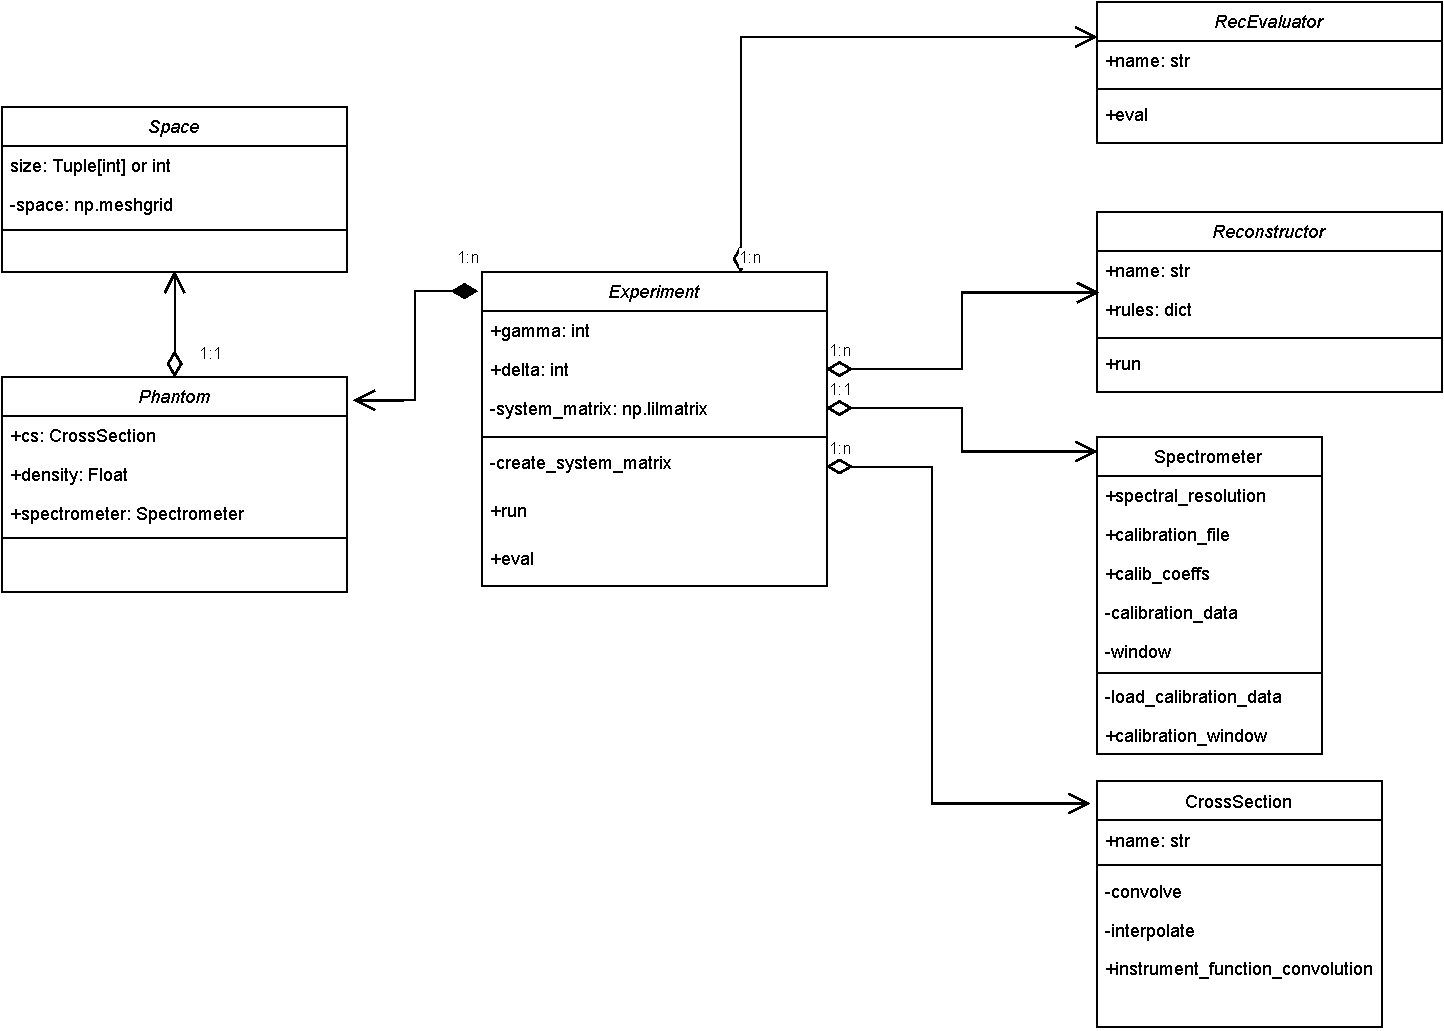
\includegraphics[width=.8\textwidth]{img/pdf/newTomosimUML.pdf}
    \caption{First draft of the \gls{uml} diagram for the new
        architectural model of the Tomosim library. Note the usage of
        several classes from the \gls{DOAS}library described in
        Section~\ref{sub:methods_ground_station}.
    }%
    \label{fig:new_tomosim_uml}
\end{figure}
